% Tests to first detection per bug, SimSpect vs AMuLeT, log scale, v2 (unified footprint corpus).
% Data (2026-11-10 11:13 UTC interim, preliminary; refresh from the final grid-timing run): simspect wiki/state/EVAL_MANIFEST.md,
% "Footprint model: the unified AMuLeT-comparison experiment". SimSpect = expected tests to first detection (N+1)/(K+1) on
% Footprint_6_u_core_lpP_fv3 at AMuLeT's configs, per-test random cache setup (warm/cold/full) and timing. UV5: K=1, extrapolated
% over the full corpus assuming only UV5-shaped tests can produce it. AMuLeT = pooled test cases (program x input) per violation,
% 32 instances x 200 programs x 140 inputs of its own fuzzer. Every text is \footnotesize (8pt).
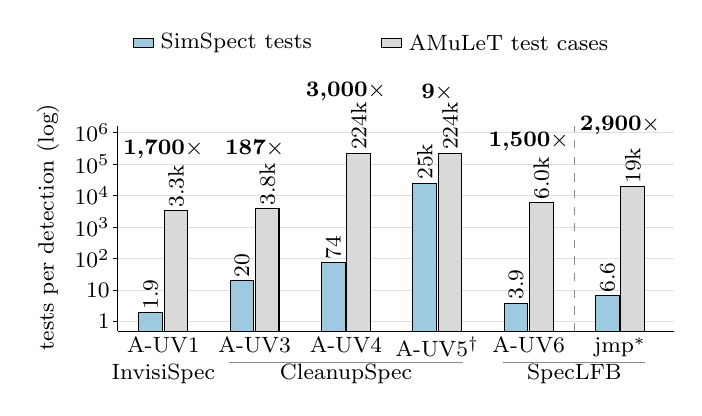
\begin{tikzpicture}[font=\footnotesize, x=1cm, y=1cm]
\definecolor{fdsim}{RGB}{158,202,225}% light blue: SimSpect
\definecolor{fdamu}{RGB}{217,217,217}% light gray: AMuLeT
\def\fdu{0.40}% cm per decade
\def\fdoff{0.30}% log10 offset so a value of 1 test still shows
\def\fdbw{0.30}% bar width, cm
\def\fdgap{1.16}% group pitch, cm
\def\fdtop{8.7}% legend height, in decades (above the tallest ratio label)
\foreach \e/\lab in {0/1, 1/10, 2/10^2, 3/10^3, 4/10^4, 5/10^5, 6/10^6} {
  \draw[black!12] (0, {(\e+\fdoff)*\fdu}) -- ({6*\fdgap+0.10}, {(\e+\fdoff)*\fdu});
  \draw (0, {(\e+\fdoff)*\fdu}) -- (-0.06, {(\e+\fdoff)*\fdu}) node[left, inner sep=1pt] {$\lab$};
}
\draw (0,0) -- (0, {(6.2+\fdoff)*\fdu});
\draw (0,0) -- ({6*\fdgap+0.10}, 0);
\node[rotate=90, anchor=south] at (-0.62, {(3+\fdoff)*\fdu}) {tests per detection (log)};
% index / log10 SimSpect / log10 AMuLeT / SimSpect label / AMuLeT label / ratio / x label
% values: UV1 1.93 vs 3,318; UV3 20.3 vs 3,794; UV4 73.5 vs 224,000; UV5 25,116 vs 224,000; UV6 3.89 vs 5,978; jmp shadow 6.62 vs 19,040
\foreach \i/\s/\a/\sl/\al/\r/\la in {
  0/0.2856/3.5209/{1.9}/{3.3k}/{1{,}700$\times$}/A-UV1,
  1/1.3075/3.5791/{20}/{3.8k}/{187$\times$}/A-UV3,
  2/1.8663/5.3502/{74}/{224k}/{3{,}000$\times$}/A-UV4,
  3/4.4000/5.3502/{25k}/{224k}/{9$\times$}/{A-UV5$^{\dagger}$},
  4/0.5899/3.7766/{3.9}/{6.0k}/{1{,}500$\times$}/A-UV6,
  5/0.8209/4.2797/{6.6}/{19k}/{2{,}900$\times$}/{jmp$^{*}$}} {
  \pgfmathsetmacro{\xc}{0.58+\i*\fdgap}
  \pgfmathsetmacro{\hs}{(\s+\fdoff)*\fdu}
  \pgfmathsetmacro{\ha}{(\a+\fdoff)*\fdu}
  \fill[fdsim] ({\xc-\fdbw-0.01}, 0) rectangle ({\xc-0.01}, \hs);
  \draw ({\xc-\fdbw-0.01}, 0) rectangle ({\xc-0.01}, \hs);
  \fill[fdamu] ({\xc+0.01}, 0) rectangle ({\xc+\fdbw+0.01}, \ha);
  \draw ({\xc+0.01}, 0) rectangle ({\xc+\fdbw+0.01}, \ha);
  % value labels, vertical, just above each bar
  \node[rotate=90, anchor=west, inner sep=1pt] at ({\xc-0.01-\fdbw/2}, \hs) {\sl};
  \node[rotate=90, anchor=west, inner sep=1pt] at ({\xc+0.01+\fdbw/2}, \ha) {\al};
  % ratio above the pair
  \pgfmathsetmacro{\hm}{max(\hs,\ha)+0.62}
  \node[anchor=south, inner sep=1pt, font=\footnotesize\bfseries] at (\xc, \hm) {\r};
  \node[anchor=north, inner sep=1.5pt] at (\xc, -0.02) {\la};
}
% defense names under their bugs
\node[anchor=north, inner sep=1.5pt] at ({0.58+0*\fdgap}, -0.36) {InvisiSpec};
\node[anchor=north, inner sep=1.5pt] at ({0.58+2*\fdgap}, -0.36) {CleanupSpec};
\node[anchor=north, inner sep=1.5pt] at ({0.58+4.5*\fdgap}, -0.36) {SpecLFB};
\draw[black!45] ({0.58+1*\fdgap-0.32}, -0.40) -- ({0.58+3*\fdgap+0.32}, -0.40);
\draw[black!45] ({0.58+4*\fdgap-0.32}, -0.40) -- ({0.58+5*\fdgap+0.32}, -0.40);
% divider before the new bug
\draw[black!45, dashed] ({0.58+4.5*\fdgap}, 0) -- ({0.58+4.5*\fdgap}, {(6.2+\fdoff)*\fdu});
% legend
\fill[fdsim] (0.20, {(\fdtop+\fdoff)*\fdu}) rectangle (0.45, {(\fdtop+0.3+\fdoff)*\fdu});
\draw (0.20, {(\fdtop+\fdoff)*\fdu}) rectangle (0.45, {(\fdtop+0.3+\fdoff)*\fdu});
\node[anchor=west, inner sep=2pt] at (0.47, {(\fdtop+0.15+\fdoff)*\fdu}) {SimSpect tests};
\fill[fdamu] (3.35, {(\fdtop+\fdoff)*\fdu}) rectangle (3.60, {(\fdtop+0.3+\fdoff)*\fdu});
\draw (3.35, {(\fdtop+\fdoff)*\fdu}) rectangle (3.60, {(\fdtop+0.3+\fdoff)*\fdu});
\node[anchor=west, inner sep=2pt] at (3.62, {(\fdtop+0.15+\fdoff)*\fdu}) {AMuLeT test cases};
\end{tikzpicture}%
